\documentclass[10pt,UTF8]{ctexart}


\usepackage[margin=2cm,a4paper]{geometry}
%\usepackage[left=0.75in,top=0.6in,right=0.75in,bottom=1.0in,a4paper]{geometry}

\setmainfont{Caladea}
%% 也可以選用其它字庫:
% \setCJKmainfont[%
%   ItalicFont=AR PL KaitiM GB,
%   BoldFont=Noto Sans CJK SC,
% ]{Noto Serif CJK SC}
% setCJKsansfont{Noto Sans CJK SC}
% \renewcommand{\kaishu}{\CJKfontspec{AR PL KaitiM GB}}

% 繁體中文
\setCJKmainfont[Path=fonts/ ]{NotoSansTC-Medium.otf}

\usepackage{minted}
\usepackage[breaklinks]{hyperref}

% Picture
% 導言區的此三行無變化
\usepackage{graphicx}
\usepackage{float} 
\usepackage{subfigure}
% 以下是新增的自定義格式更改
\usepackage[]{caption2} %新增調用的宏包
\renewcommand{\figurename}{Fig.} %重定義編號前綴詞
\renewcommand{\captionlabeldelim}{.~} %重定義分隔符
 %\roman 是羅馬數字編號,\alph是默認的字母編號,\arabic是阿拉伯數字編號,可按需替換下一行的相應位置
\renewcommand{\thesubfigure}{(\roman{subfigure})}%此外,還可設置圖編號顯示格式,加括號或者不加括號
\makeatletter \renewcommand{\@thesubfigure}{\thesubfigure \space}%子圖編號與名稱的間隔設置
\renewcommand{\p@subfigure}{} \makeatother

% Math
\usepackage {mathtools}
\usepackage{amssymb}

% Code
\usepackage{listings}
\usepackage{xcolor}
\lstset{
    % backgroundcolor=\color{red!50!green!50!blue!50},
    % 程式碼塊背景色為淺灰色
    rulesepcolor= \color{gray}, % 程式碼塊邊框顏色
    breaklines=true,  % 程式碼過長則換行
    numbers=left, % 行號在左側顯示
    numberstyle= \small,% 行號字型
    % eywordstyle= \color{red,% 關鍵字顏色
    commentstyle=\color{gray}, % 註釋顏色
    frame=shadowbox % 用方框框住程式碼塊
    }

\usepackage{hyperref}

\title{算法分析和複雜性理論}
\author{干皓丞,2101212850, 信息工程學院}

\begin{document}
\maketitle


\section{作業目標與章節摘要}

蒙地卡羅方法求圓周率 PI。

\section{作業內容概述}

作業可以從 GitHub 下的 kancheng/kan-cs-report-in-2022 專案找到,作業程式碼與文件目錄為 kan-cs-report-in-2022/AATCC/lab-report/。實際執行的環境與實驗設備為 Google 的 Colab 、MacBook Pro (Retina, 15-inch, Mid 2014) 、 Acer Aspire R7 與 HP Victus (Nvidia GeForce RTX 3060)。

本作業 GitHub 專案為 kancheng/kan-cs-report-in-2022 下的 AATCC` 的目錄。程式碼可以從 code 目錄下可以找到 *.pynb,內容包含上次課堂練習、LeetCode 範例思路整理與作業。

https://github.com/kancheng/kan-cs-report-in-2022/tree/main/AATCC

\begin{figure}[H]
\centering 

\includegraphics[width=0.30\textwidth]{aatccqr.png} 
\caption{作業專案位置}
\label{Test}
\end{figure}

1. LeetCode : https://leetcode.com/

2. LeetCode CN : https://leetcode-cn.com/

3. OnlineGDB : https://www.onlinegdb.com/ 

LeetCode 的平台部分, CN 的平台有針對簡體中文使用者進行處理,包含中英文切換等功能。OnlineGDB 則可線上進行簡易的環境測試,其程式碼涵蓋 C, C++, C\#, Java, Python, JS, Rust, Go。

\newpage

\section{作業推導}

\begin{figure}[H]
\centering 
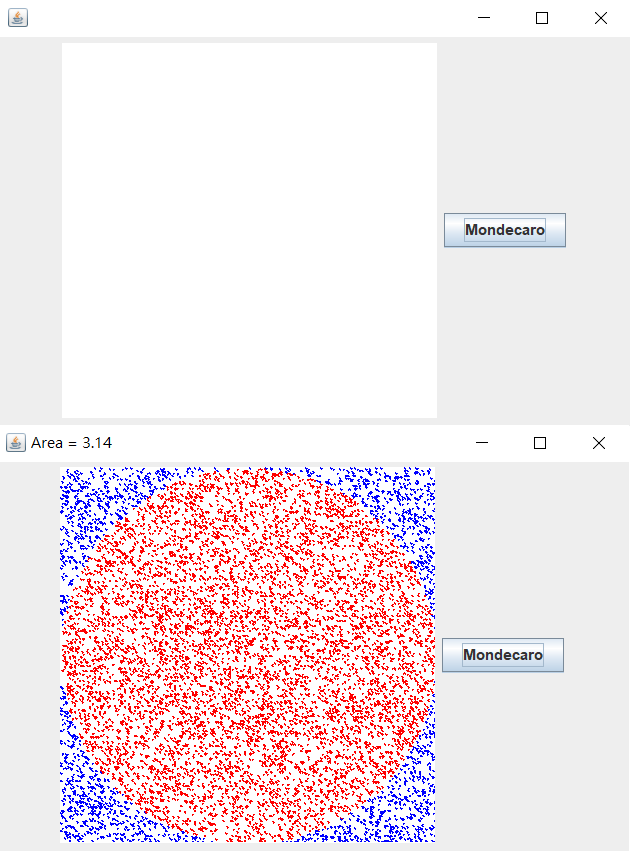
\includegraphics[width=0.85\textwidth]{w15-lab-1.png} 
\caption{Java Demo}
\label{Test}
\end{figure}

\subsection{Java 範例}

\begin{lstlisting}[language={python}]
import javax.swing.*;
import javax.swing.event.*;
import java.awt.*;
import java.awt.event.*;
import java.util.Random;
public class Mondecaro extends JFrame implements ActionListener {
    private JButton button;
    private JPanel panel;
    private int height = 300, width = 300;
    public static void main (String[] argv) {
        Mondecaro frame = new Mondecaro();
        frame.setSize(520, 350);
        frame.createGUI();
        frame.setVisible(true);
    }
    private void createGUI() {
        setDefaultCloseOperation(EXIT_ON_CLOSE);
        Container window = getContentPane();
        window.setLayout(new FlowLayout());
        panel = new JPanel();
        panel.setPreferredSize(new Dimension(width, height));
        panel.setBackground(Color.white);
        window.add(panel);
        button = new JButton("Mondecaro");
        window.add(button);
        button.addActionListener(this);
    }
    public void actionPerformed(ActionEvent e) {
        draw();
    }
    private void draw() {
        Graphics paper = panel.getGraphics();
        paper.setColor(Color.white);
        paper.fillRect( 0, 0, width, height);
        paper.setColor(Color.black);
        int px = width, py = height / 2;
        Random random = new Random ();
        int n = width / 2, in = 0, N = 10000;
        for (int i = 1; i <= N; i++) {
            int x = random.nextInt(width);
            int y = random.nextInt(width);
            double dist = Math.sqrt(Math.pow(x - n, 2) + Math.pow(y - n, 2));
            if (dist < n) {
                paper.setColor(Color.red);
                in++;
            } else {
                paper.setColor(Color.blue);
            }
            paper.drawOval( x, y, 1, 1);
            setTitle("Area = " + (double)in / i * 4);
            for (int k = 0; k < 1000; k++); 
        }
    }
}
\end{lstlisting}

\begin{lstlisting}[language={python}]
import random
total = [10, 100, 1000, 10000, 100000, 1000000, 5000000]  #隨機點數
for t in total:
    in_count = 0
    for i in range(t):
        x = random.random()
        y = random.random()
        dis = (x**2 + y**2)**0.5
        if dis<=1:
            in_count += 1
    print(t,'個隨機點時,π 是:', 4 * in_count/t)
\end{lstlisting}

結果如下 :

\begin{lstlisting}[language={python}]
10 個隨機點時,π 是: 2.8
100 個隨機點時,π 是: 3.0
1000 個隨機點時,π 是: 3.044
10000 個隨機點時,π 是: 3.1232
100000 個隨機點時,π 是: 3.15028
1000000 個隨機點時,π 是: 3.141328
5000000 個隨機點時,π 是: 3.1407488
\end{lstlisting}

\subsection{概述}

蒙特卡羅方法是一種計算方法。原理是通過大量隨機樣本,去了解一個系統,進而得到所要計算的值。
 
它非常強大和靈活,又相當簡單易懂,很容易實現。對於許多問題來說,它往往是最簡單的計算方法,有時甚至是唯一可行的方法。它誕生於上個世紀 40 年代美國的"曼哈頓計劃",名字來源於賭城蒙特卡羅,象徵概率。

\subsection{蒙特卡羅方法的應用}

通常蒙特卡羅方法可以粗略地分成兩類:

一類是所求解的問題本身俱有內在的隨機性,借助計算機的運算能力可以直接模擬這種隨機的過程。例如在核物理研究中,分析中子在反應堆中的傳輸過程。中子與原子核作用受到量子力學規律的製約,人們只能知道它們相互作用發生的概率,卻無法準確獲得中子與原子核作用時的位置以及裂變產生的新中子的行進速率和方向。科學家依據其概率進行隨機抽樣得到裂變位置、速度和方向,這樣模擬大量中子的行為後,經過統計就能獲得中子傳輸的範圍,作為反應堆設計的依據。

另一種類型是所求解問題可以轉化為某種隨機分佈的特徵數,比如隨機事件出現的概率,或者隨機變量的期望值。通過隨機抽樣的方法,以隨機事件出現的頻率估計其概率,或者以抽樣的數字特徵估算隨機變量的數字特徵,並將其作為問題的解。這種方法多用於求解複雜的多維積分問題。

\subsection{π 的計算}

第一個例子是,如何用蒙特卡羅方法計算圓周率π。正方形內部有一個相切的圓,它們的面積之比是 π/4

現在,在這個正方形內部,隨機產生 10000 個點(即 10000 個坐標對 (x, y)),計算它們與中心點的距離,從而判斷是否落在圓的內部。

如果這些點均勻分佈,那麼圓內的點應該占到所有點的 π/4,因此將這個比值乘以4,就是π的值。通過R語言腳本隨機模擬30000個點,π的估算值與真實值相差0.07\%。

\begin{figure}[H]
\centering 
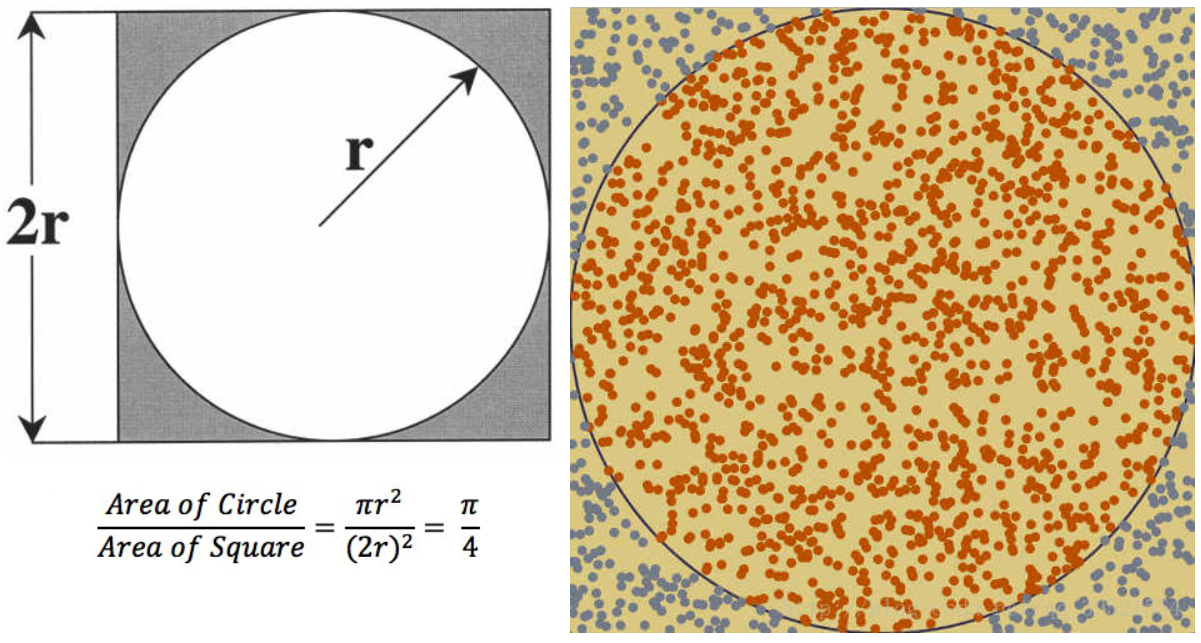
\includegraphics[width=0.95\textwidth]{w15-lab-3.png} 
\caption{PI}
\label{Test}
\end{figure}

\begin{lstlisting}[language={python}]
import numpy as np
import tqdm
#random_generate = np.random.uniform(low=0.0, high=2.0, size=(1, 1))

#求解 pi
sum = 0
for i in tqdm.tqdm(range(3000000)):
        #random_generate = np.random.rand(2
        random_generate = np.random.uniform(low=0.0, high=2.0, size=(2))
        if np.sum(np.square(random_generate-np.array([1.0, 1.0]))) <=1:
                sum += 1
print(sum)
pi = 4 * (sum / 3000000)
print('pi is:{}'.format(pi))
\end{lstlisting}

\subsection{蒙特卡羅方法求定積分}

比如積分 $\theta=\int_{a}^{b} f(x) d x$ ,如果f(x)的原函數很難求解,那麼這個積分也會很難求解。

而通過蒙特卡羅方法對其進行模擬求解的方式有二。

1. 隨機投點法

這個方法和上面的兩個例子的方法是相同的。如圖所示,有一個函數f(x),要求它從a到b的定積分,其實就是求曲線下方的面積:

這時可以用一個比較容易算得面積的矩型罩在函數的積分區間上(假設其面積為 Area),然後隨機地向這個矩形框裡面投點,其中落在函數f(x)下方的點為綠色,其它點為紅色,然後統計綠色點的數量佔所有點(紅色+綠色)數量的比例為r,那麼就可以據此估算出函數f(x)從 a 到 b 的定積分為 Area × r。

\begin{figure}[H]
\centering 
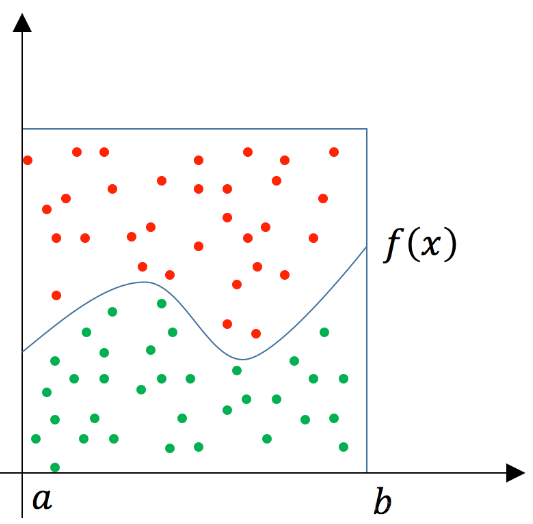
\includegraphics[width=0.40\textwidth]{w15-lab-4.png} 
\caption{隨機投點法}
\label{Test}
\end{figure}

\begin{lstlisting}[language={python}]
# 求解定積分 x^2 區間[1, 2]; 投點法
import numpy as np
import tqdm
sum = 0
for i in tqdm.tqdm(range(3000000)):

        random_generate = np.array([np.random.uniform(1, 2), np.random.uniform(0, 4)])
        if np.square(random_generate[0]) > random_generate[1]:
                sum += 1
print(sum)
area = 4 * sum / 3000000
print('Area is:{}'.format(area))
\end{lstlisting}

2. 平均值法 (期望法)

如下圖所示,在 [a,b] 之間隨機取一點 x 時,它對應的函數值就是 f(x),我們要計算 $\theta=\int_{a}^{b} f(x) d x$,就是圖中陰影部分的面積。

\begin{figure}[H]
\centering 
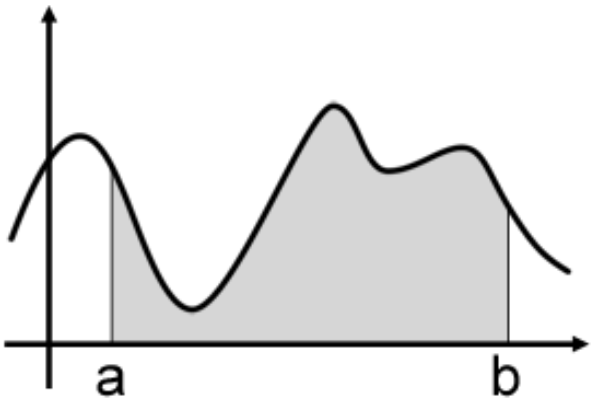
\includegraphics[width=0.40\textwidth]{w15-lab-5.png} 
\caption{陰影部分的面積}
\label{Test}
\end{figure}

一個簡單的近似求解方法就是用 $f(x) *(b-a)$ 來粗略估計曲線下方的面積,在 [a,b] 之間隨機取點 x,用 f(x) 代表在 [a,b] 上所有 f(x) 的值,如下圖所示:

\begin{figure}[H]
\centering 
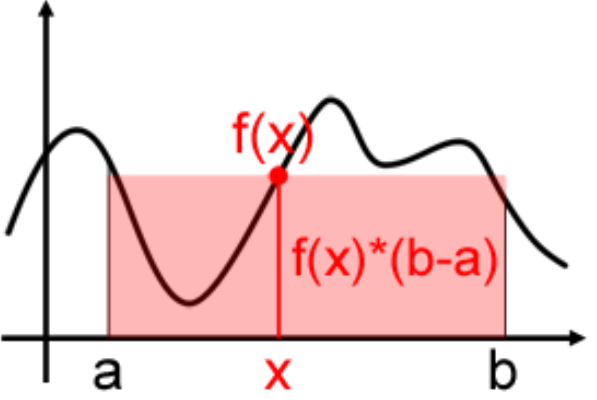
\includegraphics[width=0.40\textwidth]{w15-lab-6.png} 
\caption{近似求解方法}
\label{Test}
\end{figure}

用一個值代表 [a,b] 區間上所有的 ( ) 的值太粗糙了,我們可以進一步抽樣更多的點,比如下圖抽樣了四個隨機樣本 $x_{1}, x_{2}, x_{3}, x_{4} $ (滿足均勻分佈),每個樣本都能求出一個近似面積值 $f(x_{i}) * (b - a)$ ,然後計算他們的數學期望,就是蒙特卡羅計算積分的平均值法了。

\begin{figure}[H]
\centering 
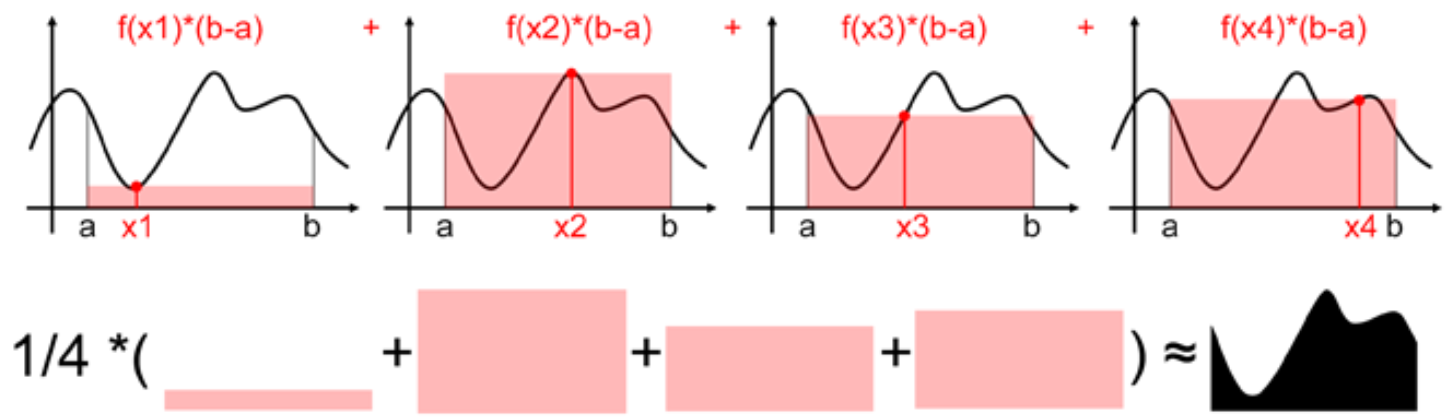
\includegraphics[width=0.90\textwidth]{w15-lab-7.png} 
\caption{近似求解方法}
\label{Test}
\end{figure}

用數學公式表述上述過程:

$S = \frac{1}{4} [f(x_{1})(b - a) + f(x_{2})(b - a) + + f(x_{3})(b - a) + + f(x_{4})(b - a)] = \frac{1}{4} (b - a)(f(x_{1}) + f(x_{2}) + f(x_{3}) + f(x_{4})) = \frac{1}{4} (b - a)\sum_{i=1}^{4} f(x_{i}) $

然後進一步我們採樣 n 個隨機樣本 (滿足均勻分佈),則有:

$S = \frac{b - a}{n} \sum_{i=1}^{n} f(x_{i})\simeq \theta$

採樣點越多,估計值也就越來越接近。

上面的方法是假定 x 在 [a,b] 間是均勻分佈的,而大多時候 x 在 [a,b] 上不是均勻分佈的,因此上面方法就會存在很大的誤差。

這時我們假設x在[a,b]上的概率密度函數為 $p(x)$ ,加入到 $\theta=\int_{a}^{b} f(x) d x$ 中變換為:

 $\theta=\int_{a}^{b} f(x) d x = \int_{a}^{b} \frac{f(x)}{p(x)} p(x) d x \simeq \frac{1}{n} \sum_{i=1}^{n} \frac{f(x_{i})}{p(x_{i})}$

這就是蒙特卡羅期望法計算積分的一般形式。那麼問題就換成瞭如何從 $p(x)$ 中進行採樣。

\begin{lstlisting}[language={python}]
# 求解定積分 X^2 區間 [1, 2]; 平均法
import numpy as np
import tqdm
sum = 0
for i in tqdm.tqdm(range(3000000)):
        random_x = np.random.uniform(1, 2, size=None)
        # None 是默認的也可以不寫
        a =  np.square(random_x)
        sum += a*(2-1)
area = sum/3000000
print('calculate by mean_average:{}'.format(area))
\end{lstlisting}

\subsection{蒙特卡洛法高維數值積分 Vegas}

高能物理研究經常要用到高維函數的數值積分。傳統的數值積分方法,比如梯形公式,辛普森積分,Gauss Quadrature 已經統統失效。原因很簡單,那些算法每個維度需要至少 M 個離散的數據點,對於 N 維積分,需要在 $M^{N}$ 個點上計算函數取值。

比如 10 維積分,每個維度用最節省的 15 個點的 Gauss Quadrature,需要計算的函數值的次數也達到了 $M^{N} = 15^{10} = 576650390625$ 約 5766 億次。

出現這種情況一般稱作維數災難。在此使用蒙特卡洛積分算法 Vegas 做高維數值積分,而 Python 的 Vegas 庫的安裝以及 Vegas 蒙卡积分的原理如下。

\subsection{VEGAS 高維函數蒙特卡洛積分}

安裝 vegas 庫很簡單,在命令行使用如下命令

\begin{lstlisting}[language={python}]
pip install vegas
\end{lstlisting}

計算如下 4 維高斯函數

$f(x_{0}, x_{1}, x_{2}, x_{3}) = N exp( - \sum_{i=0}^{3} (x_{i} - \frac{1}{2})^{2} / 0.01 )$

在閉區間 $x_{0} \in [-1, 1], x_{1} \in [0, 1], x_{2} \in [0, 1], x_{3} \in [0, 1]$

上的數值積分。其中 N = 1013.211 是一個歸一化因子。

\begin{lstlisting}[language={python}]
# copy and paste to test.py
import vegas
import math

def f(x):
    dx2 = 0
    for d in range(4):
        dx2 += (x[d] - 0.5) ** 2
    return math.exp(-dx2 * 100.) * 1013.2118364296088

integ = vegas.Integrator([[-1, 1], [0, 1], [0, 1], [0, 1]])

result = integ(f, nitn=10, neval=1000)
print(result.summary())
print('result = %s    Q = %.2f' % (result, result.Q))
\end{lstlisting}

\begin{lstlisting}[language={python}]
itn   integral        wgt average     chi2/dof        Q
-------------------------------------------------------
  1   1.04(69)        1.04(69)            0.00     1.00
  2   0.83(31)        0.87(28)            0.08     0.78
  3   1.10(25)        1.00(19)            0.24     0.79
  4   0.922(74)       0.932(69)           0.21     0.89
  5   1.052(62)       0.999(46)           0.58     0.68
  6   0.965(27)       0.974(23)           0.54     0.74
  7   0.996(21)       0.986(16)           0.53     0.78
  8   0.982(17)       0.984(12)           0.46     0.86
  9   1.002(15)       0.9910(92)          0.51     0.85
 10   0.998(12)       0.9934(74)          0.48     0.89

result = 0.9934(74)    Q = 0.89
\end{lstlisting}

可以看到 result.summary() 返回了 10 次迭代的結果。

如果只想返回最終結果,去掉 summary(),

EX : result = 1.0101(93)

result 是一個 gvar 類型的數,括號裡的數表示誤差

- 使用 result.mean 返回均值 1.0101

- 使用 result.sdev 返回不確定部分 0.0093

如果積分變量 x[1] 的積分上限依賴積分變量 x[0], 如

$\int_{0}^{1} d x_{0} \int_{0}^{x_{0}} d x_{1} \sin(x_{0}x_{1})$

被積函數可以這樣寫

\begin{lstlisting}[language={python}]
def f(x):
    if x[1] > x[0]: return 0
    return sin(x[0]*x[1])
\end{lstlisting}


\subsection{蒙特卡洛積分 - 重要抽樣法}

這裡忽略黎曼積分的適用性以及勒貝格積分的優越性討論,來自 Mathematica 關於黎曼求和、黎曼積分的例子

\begin{figure}[H]
\centering 
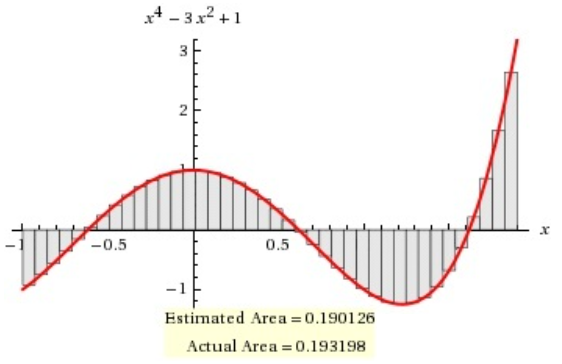
\includegraphics[width=0.90\textwidth]{w15-lab-8.png} 
\caption{Mathematica 關於黎曼求和、黎曼積分的例子}
\label{Test}
\end{figure}

黎曼積分 原理指導我們,為了求一維函數 f(x) 在閉區間 [a, b] 上的定積分,可以先把區間分成 n 份, $a<x_{1}<x_{2}<\cdots<x_{n-1}<b$  , 其中格子大小為 $\Delta x_{i}=x_{i+1}-x_{i}$

函數的積分近似等於小格子中任一處的函數值 $f\left(x_{i}^{*}\right)$ 乘以 $\Delta x_{i}$ ,並對所有格子求和。

$F \approx \sum_{i} f\left(x_{i}^{*}\right) \Delta x_{i}$

因此可以使用均勻分佈抽樣出的 $x_{i}$ 點上函數值 $f(x_{i})$ 乘以平均間距 $\frac{x_{max}-x_{min}}{N}$ 求和來近似黎曼積分。

$F=\int_{x_{\min }}^{x_{\max }} f(x) d x \approx \frac{x_{\max }-x_{\min }}{N} \sum_{i=1}^{N} f\left(x_{i}\right)$

如果是高維積分,只需要把右邊的 $x_{max} - x_{min}$ 換成體積 $\mathcal{V}$ , 積分公式變為,

$F \approx \frac{\mathcal{V}}{N} \sum_{i}^{N} f\left(x_{i}\right) \approx \mathcal{V} \mathrm{E}\left[f\left(x_{i}\right)\right] $

其中 $\mathrm{E}[f]$ 表示 $f$ 在均勻分佈下的期望值。

馬文淦的《計算物理》中介紹,根據中心極限定理,因為 F 是大量隨機變量 $f(x_{i})$ 的求和,它的值滿足正態分佈。

蒙卡積分的誤差 $\propto \frac{\sigma\left(f_{x_{i}}\right)}{\sqrt{n}}$ ,因此有兩種辦法可以提高蒙特卡洛積分的精度。

第一種是多撒點,將撒點個數 $n$ 每增加 100 倍,蒙卡积分的誤差就會減小為原來的十分之一。這個結論獨立於積分的維數。

第二種是減小 $x_{i}$ 點上集合 $\left\{f\left(x_{i}\right)\right\}$ 的漲落 $\propto (f x_{i})$ 。

如果 $f(x) = c$ 是常數,則集合 $\left\{f\left(x_{i}\right)\right\}$ 的方差最小,為 $\sigma^{2}=\left\langle(f-\langle f\rangle)^{2}\right\rangle=0$ 。

當 $f(x)$ 偏離均勻分佈,在局部有很尖的峰,則集合  $\left\{f\left(x_{i}\right)\right\}$ 的方差 (漲落) 就會比較大。

減小被積函數方差的方法是選擇一個與 $f(x)$ 形式相近,但比較好抽樣的函數 $g(x)$, 將積分寫為,

$F=\int_{\mathcal{V}} \frac{f(x)}{g(x)} g(x) d x=\mathcal{V} \mathbb{E}_{g}\left[\frac{f(x)}{g(x)}\right] $

其中期望值 $\mathbb{E}_{g}$ 表示按照概率密度函數 $g(x)$ 抽樣出一系列點 $x_{i}$ ,並使用這些點計算 $f(x)/g(x)$ 的均值,

$\frac{1}{N} \sum_{i}^{N} \frac{f\left(x_{i}\right)}{g\left(x_{i}\right)}$

此時,因為 $f(x) ~ g(x)$ ,被積函數 $f(x)/g(x) ~ 1$ 接近常數, $\left\{f\left(x_{i}\right) / g\left(x_{i}\right) \right\}$ 方差更小,從理論上降低蒙卡积分的誤差。

與暴力增加 n 相比, $g(x)$ 函數的具體形式依賴於被積函數。

Vegas 積分就是要使用適配的方式,自動尋找 g(x)。

\subsection{自適應方法做重要抽樣}

VEGAS 積分有兩個版本。經典版本 VEGAS 與進化版本 VEGAS+。下面是 VEGAS+ 文章的摘要。

We describe a new algorithm, VEGAS+, for adaptive multidimensional Monte Carlo integration. The new algorithm adds a second adaptive strategy, adaptive stratified sampling, to the adaptive importance sampling that is the basis for its widely used predecessor VEGAS. Both VEGAS and VEGAS+ are effective for integrands with large peaks, but VEGAS+ can be much more effective for integrands with multiple peaks or other significant structures aligned with diagonals of the integration volume. We give examples where VEGAS+ is 2-17 times more accurate than VEGAS. We also show how to combine VEGAS+ with other integrators, such as the widely available MISER algorithm, to make new hybrid integrators. For a different kind of hybrid, we show how to use integrand samples, generated using MCMC or other methods, to optimize VEGAS+ before integrating. We give an example where preconditioned VEGAS+ is more than 100 times as efficient as VEGAS+ without preconditioning. Finally, we give examples where VEG AS+ is more than 10 times as efficient as MCMC for Bayesian integrals with D = 3 and 21 parameters. We explain why VEGAS+ will often outperform MCMC for small and moderate sized problems.

原始 VEGAS 積分將積分區域分成 N 份,然後動態調整每份的寬度 $\Delta x_{i} $ ,使得 $f\left(x_{i}\right) \Delta x_{i} $ 的值趨於常數。即

$f\left(x_{0}\right) \Delta x_{0} \approx f\left(x_{1}\right) \Delta x_{1} \approx \ldots \approx f\left(x_{n}\right) \Delta\left(x_{n}\right)=\text { const }$

這種方法使 $f(x)$ 值較大的地方,格子分的細,$f(x)$ 值較小的地方,格子分的粗。從而完成重要抽樣的目的,減小積分誤差。原始 VEGAS 積分對於峰值平行於自變量方向的函數比較有效。如果被積函數有多個峰值,則會產生很多 "假峰" 區域。

\begin{figure}[H]
\centering 
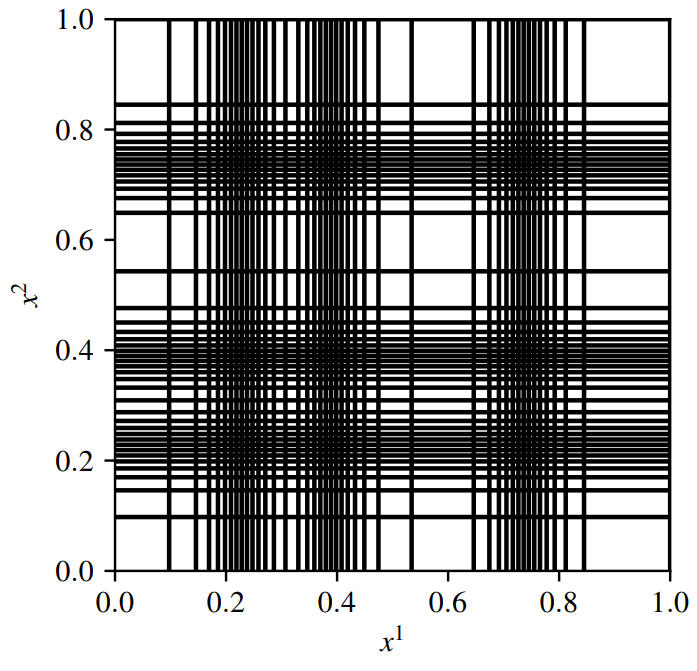
\includegraphics[width=0.90\textwidth]{w15-lab-9.png} 
\caption{假峰}
\label{Test}
\end{figure}

比如二維積分,有 3 個峰值,區域在紅色圓圈附近,根據原始 VEGAS 積分的自適應方法,會額外產生 6 個"假峰",用藍色 x 標記,被積函數 $f(x^{1}, x^{2})$ 在這些區域的值接近於 0,而自適應方法會在這 6 個區域產生很多積分點,導致 原始 VEGAS 積分效率低下。

在高維積分中,如果被積函數有多個對角峰值,情況會更加嚴重。比如 10 維下的 3 對角峰值,這樣的 "假峰" 會有 $3^{10} - 3$ 個。

進化版 VEGAS+ 額外加入自適應分層抽樣 Adaptive Stratified Integration。

將積分區域分成很多小的超立方 cube,如果某個 cube 中的積分值多次迭代方差較大,就將區域細分。做多個峰值的積分更高效,比原始版本精度提高 2 到 17 倍。這種方法別的很多地方用到,比如 MISER,FOAM,ZMCIntegral 等。

\begin{figure}[H]
\centering 
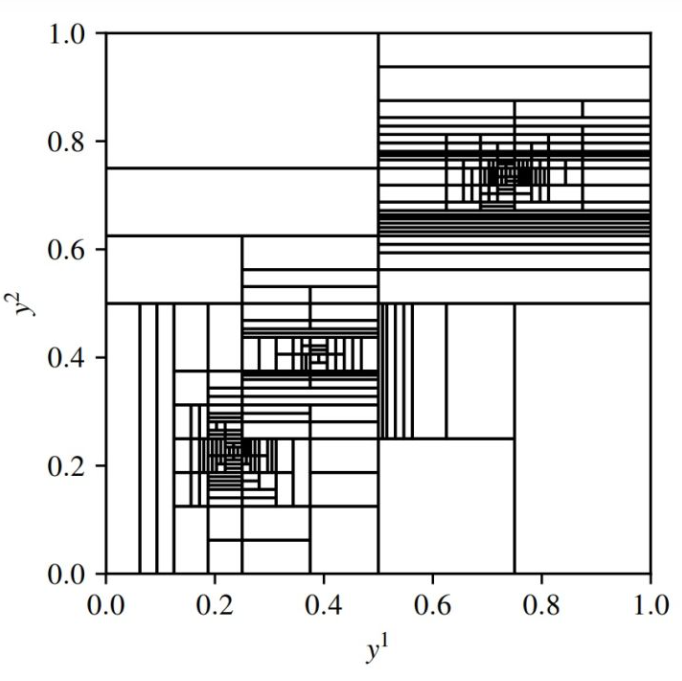
\includegraphics[width=0.90\textwidth]{w15-lab-10.png} 
\caption{MISER 自適應分層抽樣法}
\label{Test}
\end{figure}

自適應重要抽樣加分層抽樣法加成的 VEGAS+ 在多個高維積分任務上都表現不錯。另外,2009年的文章還提到一種新方法,使用馬爾科夫鏈蒙特卡洛 MCMC 先尋找被積函數的峰值位置,預產生一些積分位置,然後送入 VEGAS+ 中,可以比從零開始的 VEGAS+ 加速 100 倍。

\section{Reference}

1. MIT 6.0002 Introduction to Computational Thinking and Data - Monte Carlo Simulation : 

https://www.youtube.com/watch?v=OgO1gpXSUzU

2. 蒙特卡洛原理代碼 monte carlo :

https://blog.csdn.net/yjinyyzyq/article/details/86600393

3. 蒙特卡洛法高維數值積分 Vegas :

https://zhuanlan.zhihu.com/p/264315872

4. 一文詳解蒙特卡洛(Monte Carlo)法及其應用 :

https://blog.csdn.net/qq\_39521554/article/details/79046646

5. https://www.scratchapixel.com/lessons/mathematics-physics-for-computer-graphics/monte-carlo-methods-in-practice/monte-carlo-integration

6. 蒙特卡羅方法詳解 : https://zhuanlan.zhihu.com/p/369099011

7. https://en.wikipedia.org/wiki/Monte\_Carlo\_method

8. https://github.com/gplepage/vegas

9. https://vegas.readthedocs.io/en/latest/

10. https://arxiv.org/abs/2009.05112

11. vegas 原始文獻:G. P. Lepage, J. Comput. Phys. 27(1978) 192.
%\section{附錄}

% 數學意義說明

% $$\min \limits_{G}\max \limits_{D}{V_I(D,\ G)=V(D,G)-\lambda L_I(G,Q)}$$

%	\begin{lstlisting}[language={python}]

%	\end{lstlisting}

%\begin{enumerate}
%\item Y
%\item A
%\end{enumerate}

% \newpage

\clearpage

\end{document}